%!TEX TS-program = xelatex
%!TEX encoding = UTF-8 Unicode

\documentclass[12pt]{elsarticle}
\usepackage{geometry}
\usepackage{amsmath}
\geometry{letterpaper}

\usepackage{multirow}
\usepackage{fontspec,xltxtra,xunicode}
\defaultfontfeatures{Mapping=tex-text}
\setromanfont{STKaiti} %设置中文字体
\XeTeXlinebreaklocale “zh”
\XeTeXlinebreakskip = 0pt plus 1pt minus 0.1pt %文章内中文自动换行


\begin{document}

\begin{frontmatter}
\title{\textbf{ECG数据分类统计学习实验报告}}
\author{学号:115033910014   \\
姓名:解加鹏 \\
导师:吴帆}
   
\begin{abstract}
特征提取在提高分类的准确性中起着关键作用,本次报告将使用基于模型的特征提取方法,用AR模型刻画ECG数据,然后提取模型的系数作为特征矢量去进行分类。提取完特征以后可以用高斯核的支持向量机(SVM)和KNN对数据进行分类。我们通过交叉验证来确定模型的参数,以选择最适合的模型。结果显示SVM的分类效果明显好于KNN。
\end{abstract}
\end{frontmatter}
\section{数据处理}
在本次试验中,数据为心电图ECG数据,首先需要对数据进行初步处理。对于ECG数据,通常采用AR模型进行特征提取。AR模型是一个线性的,二阶矩平稳模型,比较适合端数据分析。今年来的研究表明,AR模型比ARMA模型更具优势,用AR模型进行特征提取时,识别率非常高。下面简要介绍一下AR模型的原理。
\subsection{$AR(p)$模型}
许多观测时间序列都表现出连续的自相关性,即观测数据之间存在线性联系。这表明已经观察到的数据可以预测当前的观察数据。自回归模型(AR)将当前的观测$y_t$建模为过去p个数据$y_{t-1},y_{t-2},...,y_{t-p}$的函数。称一个依赖过去p个观测值的AR模型的度数为p,记做$AR(p)$。$AR(p)$模型的形式如下
\begin{align}
y_t = c + \phi_1y_{t-1}+...+\phi_{p}y_{t-p}+\varepsilon_t \notag
\end{align}
这里$\varepsilon_t$表示一个期望为0的白噪音。用滞后算子多项式符号来表示,$L^iy_t=y_{t-i}$。定义p度AR滞后算子多项式$\phi(L)=(1-\phi_1L-...-\phi_pL^p)$.AR模型可以写成:
\begin{align}
\phi(L)y_t = c+\varepsilon_t \notag
\end{align}
AR滞后算子多项式里面系数的符号和原来的符号正好相反,在Ecnometrics Toolbox里面用原来系数的符号。解上式可以看出,
\begin{align}
&\phi(L)y_t = c+\varepsilon_t \notag\\
&y_t = \mu+\phi^{-1}(L)\varepsilon_t = \mu+\psi(L)\varepsilon_t \notag
\end{align}
其中$\mu = \frac{c}{1-\phi_1-...-\phi_p}$.
\begin{table}[!htbp]
\centering
\begin{tabular}{|c|c|}
\hline
$order\ of\ cofficients$ & accuracy\%\\
\hline
p=40 & 69 \\
\hline
p=45 & 72 \\
\hline
p=50 & 78 \\
\hline
p=55 & 77 \\
\hline
\end{tabular}
\end{table}

经过试验,本次数据处理使用的p为50。因此对于每一个样本,提取特征以后的数据维数是50*12=600维。提取完特征以后,下面使用SVM和KNN对数据进行分类。在原数据中,样本的label对应心脏病的症状,分别是窦性心律-电轴左偏,窦性心律-完全性左束支传导阻滞,窦性心律-提示左室肥厚,正常心电图,窦性心律-完全性右束支传导阻滞,窦性心动过缓,为了方便表述,在本文中将分别使用1,2,3,4,5,6来代替。下面简单介绍SVM和KNN的原理。

\subsection{SVM}
在机器学习领域,支持向量机SVM(Support Vector Machine)是一个有监督的学习模型,通常用来进行模式识别、分类、以及回归分析。它是一种二类分类模型,其基本模型定义为特征空间上的间隔最大的线性分类器,其学习策略便是间隔最大化,最终可转化为一个凸二次规划问题的求解。SVM的主要思想可以概括为两点:⑴它是针对线性可分情况进行分析,对于线性不可分的情况,通过使用非线性映射算法将低维输入空间线性不可分的样本转化为高维特征空间使其线性可分,从而 使得高维特征空间采用线性算法对样本的非线性特征进行线性分析成为可能.SVM具有如下的特征:

⑴SVM学习问题可以表示为凸优化问题,因此可以利用已知的有效算法发现目标函数的全局最小值。而其他分类方法(如基于规则的分类器和人工神经网络)都采用一种基于贪心学习的策略来搜索假设空间,这种方法一般只能获得局部最优解。

⑵SVM通过最大化决策边界的边缘来控制模型的能力。尽管如此,用户必须提供其他参数,如使用核函数类型和引入松弛变量等。

⑶通过对数据中每个分类属性引入一个哑变量,SVM可以应用于分类数据。

本文使用开源的LIBSVM作为求解SVM的工具。
\subsection{KNN}
邻近算法,或者说K最近邻(kNN,k-NearestNeighbor)分类算法是数据挖掘分类技术中最简单的方法之一。所谓K最近邻,就是k个最近的邻居的意思,说的是每个样本都可以用它最接近的k个邻居来代表。kNN算法的核心思想是如果一个样本在特征空间中的k个最相邻的样本中的大多数属于某一个类别,则该样本也属于这个类别,并具有这个类别上样本的特性。该方法在确定分类决策上只依据最邻近的一个或者几个样本的类别来决定待分样本所属的类别。 kNN方法在类别决策时,只与极少量的相邻样本有关。由于kNN方法主要靠周围有限的邻近的样本,而不是靠判别类域的方法来确定所属类别的,因此对于类域的交叉或重叠较多的待分样本集来说,kNN方法较其他方法更为适合。

\section{模型选择及分类}
\subsection{SVM}
借助于LIBSVM,我们可以很轻松的实现SVM,通过如下函数,可以求得对应SVM问题的解

model\ = svmtrain(training-label-vector,\ training-instance-matrix)

[predict-label,\ accuracy, dec-values]\ =\ svmpredict(data-label,\ data-inst)

我们使用径向基函数(Radial\ basis\ function)作为SVM的核,可选参数是罚项的系数C和RBS里面的$\gamma$,利用交叉验证的方法,可以确定最优的参数。我们做了几组实验来估计泛化误差,其中C从5到50,$\gamma$从$2^{-3}$到$2^{-12}$,结果如下图(附件有原始数据):
\begin{figure}[!ht]
  %\vspace{-0.08in}
  \centering
  % Requires \usepackage{graphicx}
  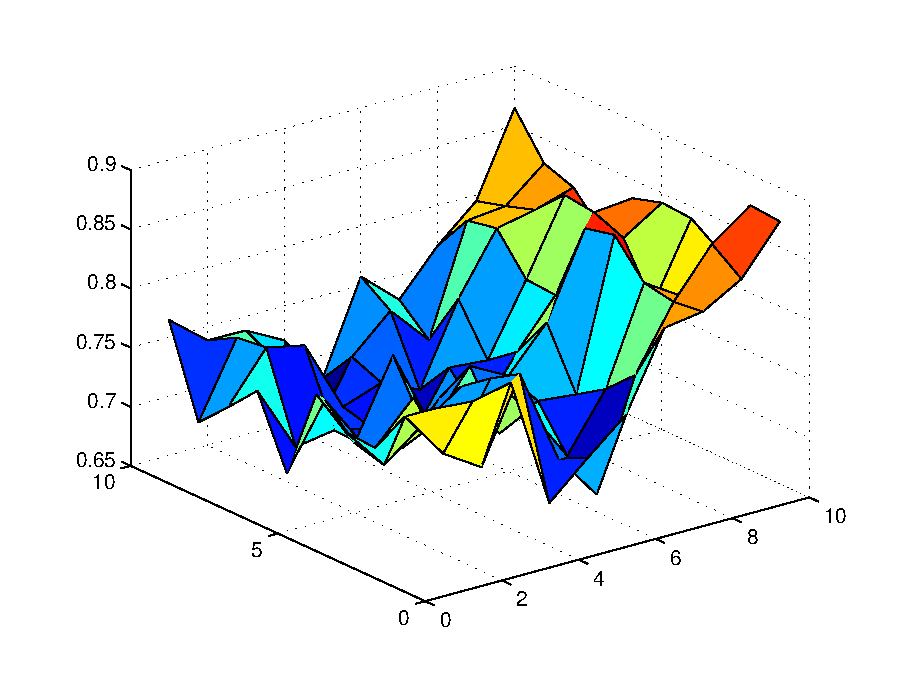
\includegraphics[width=10cm]{svm}\\
  %\vspace{-0.08in}
  \caption{SVM}\label{fig:delay}
  %\vspace{-0.05in}
\end{figure}
可见SVM的正确率可以达到85$\%$以上。
\subsection{KNN}
邻近算法,或者说K最近邻(kNN,k-NearestNeighbor)分类算法是数据挖掘分类技术中最简单的方法之一。所谓K最近邻,就是k个最近的邻居的意思,说的是每个样本都可以用它最接近的k个邻居来代表。matlab自带了KNN的分类算法,调用方法如下:

knnclassify(test-data,\ train-data,\ train-label,\ k)

同样,我们使用交叉验证的方法测试不同的k,k从10到500,结果如下(附件有原始数据),
\begin{figure}[!ht]
  %\vspace{-0.08in}
  \centering
  % Requires \usepackage{graphicx}
  \includegraphics[width=10cm]{knn}\\
  %\vspace{-0.08in}
  \caption{knn}\label{fig:delay}
  %\vspace{-0.05in}
\end{figure}

可见KNN的正确率可以达到60$\%$并收敛。效果比SVM差,原因可能是训练样本的数量比较少,还有样本特征维度比较高。


\subsection{小结}
从上面的数据可以看出,经过AR的特征提取,在选择了适当的参数之后,SVM和KNN都可以取得比较好的结果。


\section{LDA降维和PCA降维}
编写了LDA降维和PCA的代码之后,我对训练数据整体进行了降维。降到2维之后,根据最优投影矩阵,投影结果如下图。
\begin{figure}[!ht]
  %\vspace{-0.08in}
  \centering
  % Requires \usepackage{graphicx}
  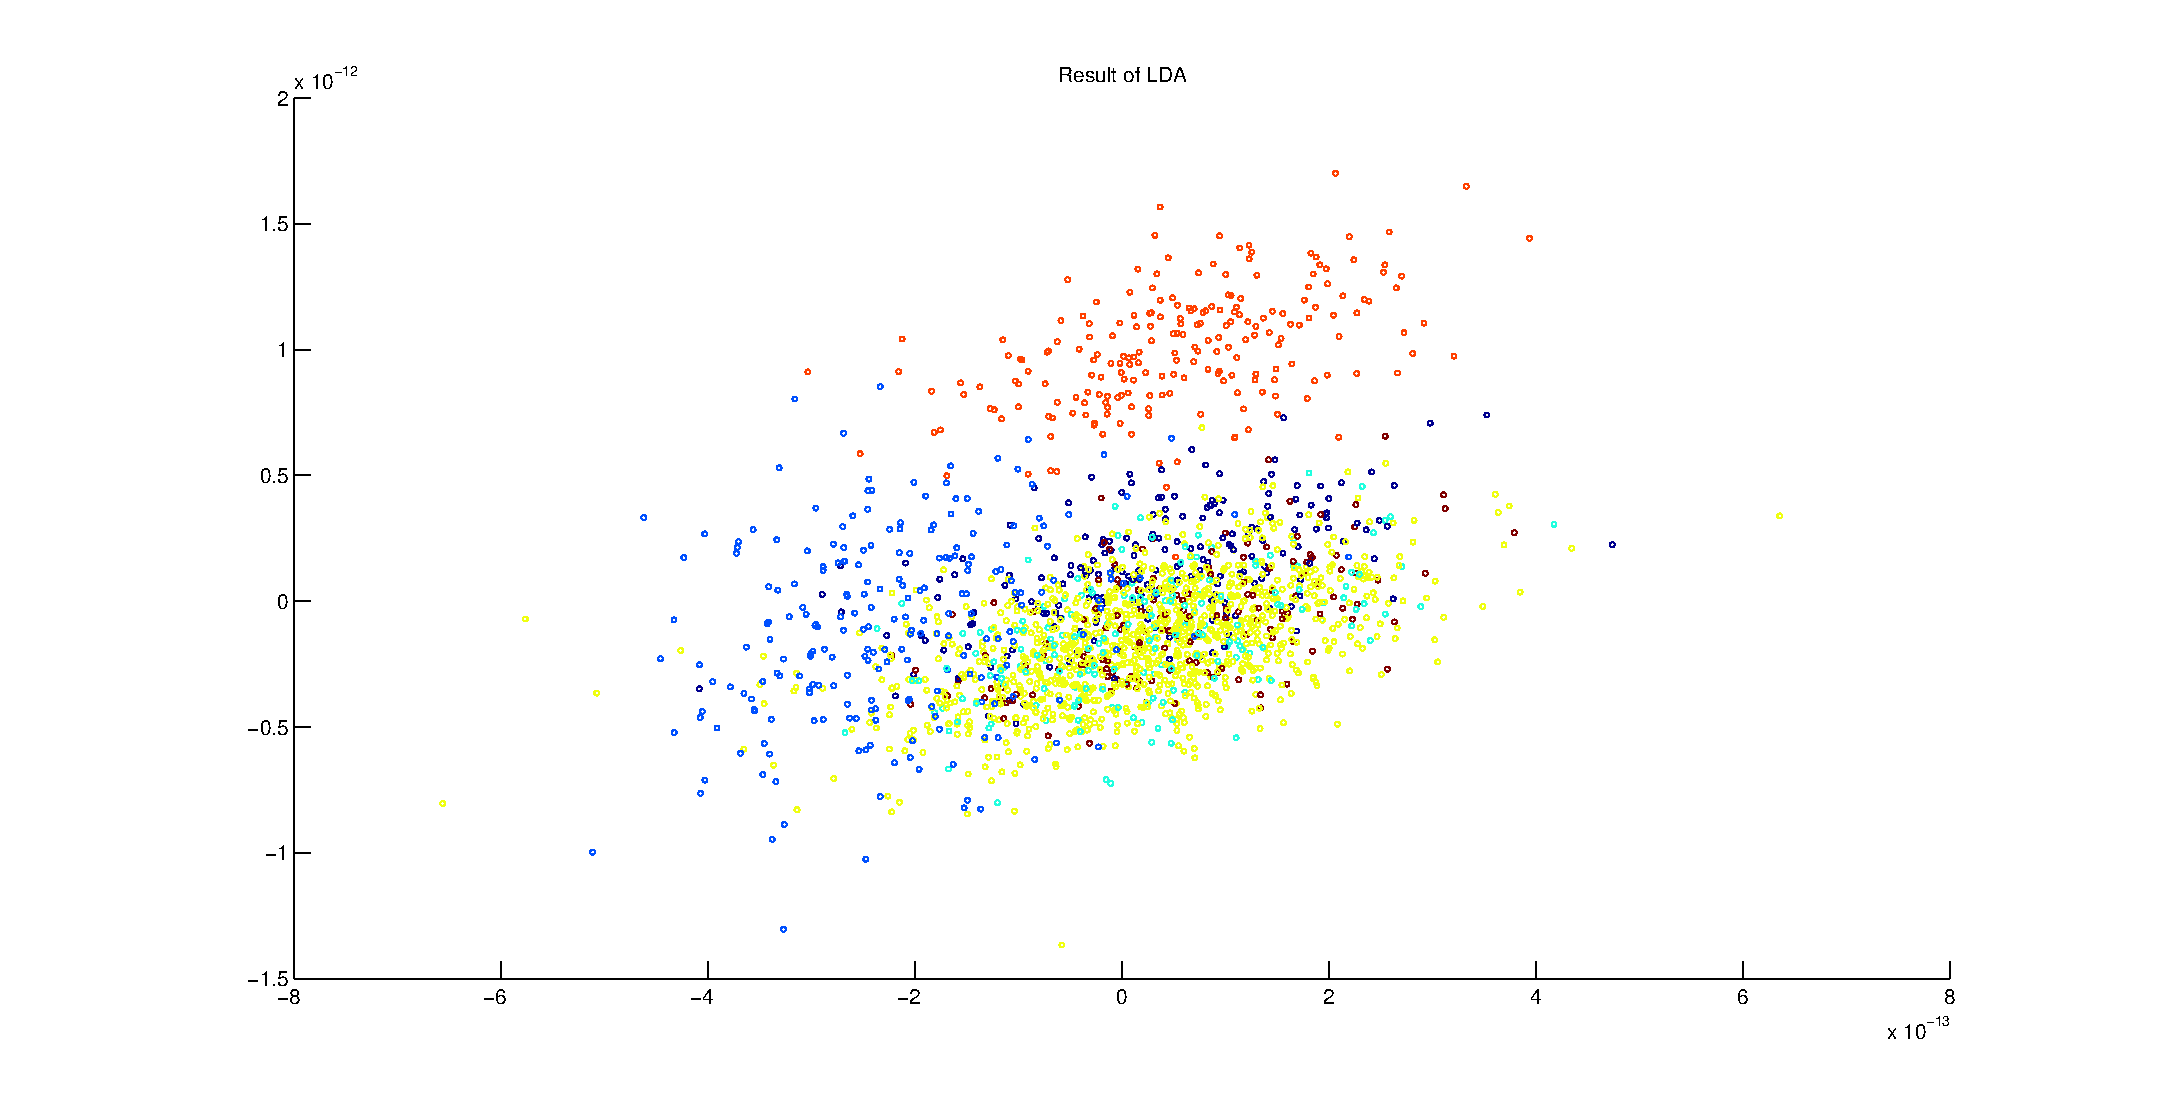
\includegraphics[width=15cm]{lda}\\
  %\vspace{-0.08in}
  \caption{lda}\label{fig:delay}
  %\vspace{-0.05in}
\end{figure}

\begin{figure}[!ht]
  %\vspace{-0.08in}
  \centering
  % Requires \usepackage{graphicx}
  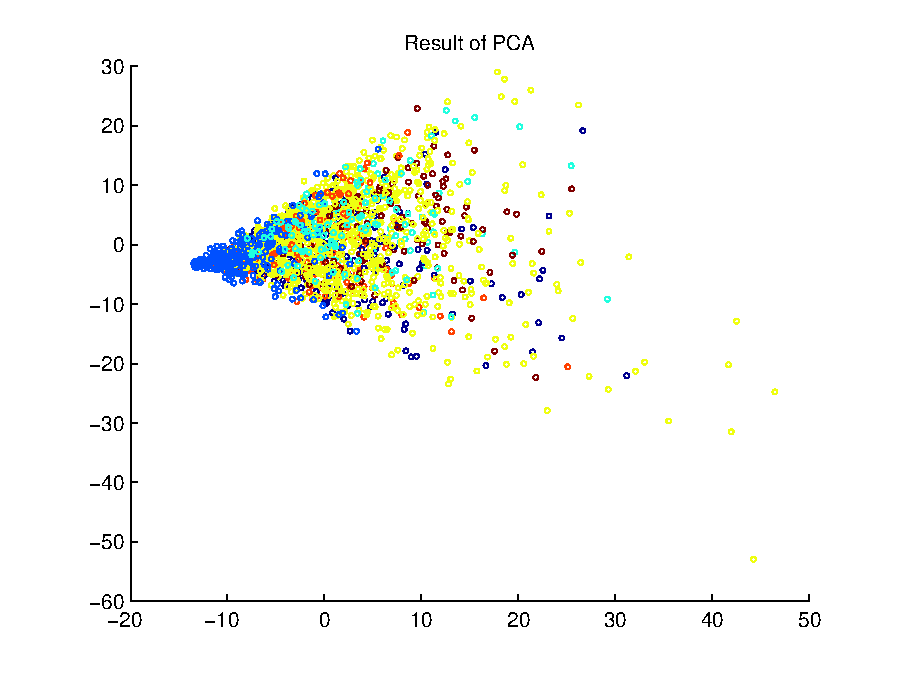
\includegraphics[width=15cm]{pca}\\
  %\vspace{-0.08in}
  \caption{pca}\label{fig:delay}
  %\vspace{-0.05in}
\end{figure}

在原始的高维空间中,包含有冗余信息以及噪音信息,在实际应用例如图像识别中造成了误差,降低了准确率;而通过降维,我们希望减少冗余信息所造成的误差,提高识别(或其他应用)的精度。又或者希望通过降维算法来寻找数据内部的本质结构特征。我们看到将数据投影到2维以后仍然有较大的重叠,但是LDA的分离效果比PCA的分离效果好。



\end{document}

